\documentclass{article}
\usepackage{graphicx}
\usepackage[utf8]{inputenc}

\title{Reto 1}
\author{Luisa Contreras\\Jairo Vanegas\\ Nicolas Quintero \\Gabriel Forero }
\date{Septiembre 2020}

\usepackage{natbib}
\usepackage{graphicx}

\begin{document}

\maketitle

\section{Evaluación de un Polinomio}
\subsection{Implementación del algoritmo de Horner }
\subsubsection{Primera Derivada}
El método de Horner, es un método que permite evaluar un polinomio de forma monomio, es decir que lo realiza por medio de multiplicaciones y sumas. Por lo tanto, para hallar Horner en la primera derivada del polinomio se utilizó la división sintética. Lo primero que se realizo fue la comprobación y cancelación de coeficientes en este se busca seleccionar y eliminar los números son suficientemente pequeños, para convertirlos en cero con el fin de que estos no intervengan con el resultado, esto lo realizamos encontrando los valores más pequeños, ubicamos su posición y finalmente convertimos el valor de esta posición en cero. Luego de ello se aplica la división sintética, como ya lo mencionamos, que se realiza reduciendo el primer término, luego multiplicándolo y por último almacenándolo, de esta manera se realiza recursivamente hasta haber divido cada monomio.  
\subsubsection{Segunda Derivada}
Horner nos permite encontrar el valor de una función en un punto determinado garantizando que el número máximo de operaciones corresponde al grado del polinomio. Para la segunda derivada se implementó un arreglo de valores reales donde el índice de la posición.
El algoritmo de Horner nos permite encontrar el valor de una función en un punto determinado para asegurar que el número máximo de operaciones y el orden del polinomio considera una serie de valores para su realización.  Para lograr su implementación se realiza un arreglo de número reales donde el índice de la posición, que se logra entender de la siguiente manera:

$P(x)=a_0X^{n} + a_1X^{n-1}+a_2X^{n-2}+a_3X^{n-3}+...+a_nX^{0}$

$[a_0 ]       [a_1 ]        [a_2 ]       [a_3 ]          …       [a_n ]$

Partiendo de ello, se implementaron un algoritmo que corresponde a la implementación de las derivadas. La función opera el arreglo antes mencionado de la forma $P(x)=a_0X^{n} + a_1X^{n-1}+a_2X^{n-2}+a_3X^{n-3}+...+a_nX^{0}$ donde cada monomio es derivado por medio de la regla de derivación $n*aX^(n-1)$ ,  para después ser sumado. Por esto, se tomó en cuenta que al realizar esta operación que el tamaño del arreglo es variable, entonces después de dicha operación se toma en cuenta que n no es igual al tamaño del arreglo si no, que será de $n=|Coheficientes|-1$ . 
Finalmente se obtiene un nuevo arreglo que contendrá los coeficientes de la función derivada y con esta se ejecuta el algoritmo de Horner nuevamente y obtendremos el resultado de la derivada del polinomio evaluado en un punto $X_i$.
\subsection{Newton-Horner}
Para el método de Newton se usa para calcular las raíces de un polinomio. Definida por una función derivable definida en los reales. Donde comenzamos con $X_0$ como valor inicial y definimos para cada número n, la siguiente recursión:

$X_{n+1}=X_n-\frac{f(X_n)}{f'(X_n)}$

Ya considerando ello usaremos Newton para calcular una raíz del polinomio y dividiremos el polinomio con el método primer método de Horner, ya definido. Para el orden de convergencia se tienen dos variables, en las cuales, en una se tiene cuantas veces se usa Horner en el algoritmo y cuantas veces el algoritmo recurre. De esta forma se almacenan de acuerdo van sucediendo luego de cada iteración y de cada proceso para poder determinar las iteraciones totales y las iteraciones del método propio. 
\section{Algoritmo de Brent}
El algoritmo de Brent busca las raíces de una función combinando tres métodos: Bisección, Secante e interpolación lineal. Logrando tener la confiabilidad de bisección, en menor cantidad de tiempo. A continuación, se explicará como se usó el algoritmo de Brent para encontrar las raíces de la función: 

$F(x)=X^{3}-2X^{2}+\frac{4X}{3}-\frac{8}{27}$

Para comprobar la veracidad del método se usó Wólfram con el fin de obtener la respuesta y así poder compararlo con el algoritmo de Brent. Teniendo como resultado que la raíz es:

$X=\frac{2}{3}$
\subsection{Seudocódigo}
El algoritmo de Brent se implementó en Python, a continuación, se muestra el seudocódigo:

Se definen los intervalos de la función [a,b]

Calcular f(a)

Calcular f(b)

if f(a)*f(b)$\geq$ 0 then 

  Sale de la función por que la raíz no esta en el intervalo
  
end if

if $|f(a)|$ $\leq$ $|f(b)|$ then

  Se intercambian los valores a y b
  
end if

c = a

repeat until f(b) = 0 or f(s) = 0 or $|b-a|$ $\geq$ tolerancia (converge)

  if f(a) 	$\neq$ f(c) and f(b) $	\neq$ f(c) then
  
     s= Se usa la formula de la interpolación lineal para calcular la raiz 
     
  else
  
     	s= Se usa la formula de la secante para calcular la raiz 
     	
  end if
  
  if  s is not between $\frac{3a+b}{4}$ and b or
  
     ($|s-b|$ $\geq$  $\frac{|b-c|}{2}$) or
     
     ($|s-b|$ $\geq$  $\frac{|c-d|}{2}$) or
     
     ($|b-c|$ $\leq$  $|s|$) or
     
     ($|c-d|$ $\leq$  $|s|$) then
     
      s=Se usa la formula del metodo  bisección para calcular la raiz
      
  end if
  
  calculate f(s)
  
  d = c  (d no se usa en la primera iteración)   
  
  c = b

  if f(a)*f(s) $\leq$  0 then
  
    b = s 
    
  else
  
    a = s 
    
  end if

  if $|f(a)|$ $\leq$ $ |f(b)|$ then
  
    Se intercambian los valores a y b
    
  end if
  
end repeat

La raíz se encuentra en el valor de s


\subsection{Resultados}
Los resultados que se obtuvieron con una tolerancia de $\epsilon^{-14}$ fueron los siguientes: 

\begin{tabular}{| c | c |}
\hline
Iteración & Raíz \\ \hline
1 & -0,007936507936508 \\
2 & 0,488095238095238 \\
3 & 0,736111111111111 \\
4 & 0,612103174603174 \\
5 & 0,674107142857142 \\
6 & 0,643105158730158 \\
7 & 0,658606150793650 \\
8 & 0,666356646825397 \\
9 & 0,670231894841270 \\
10 & 0,668294270833333 \\
11 & 0,667325458829365 \\
12 & 0,666841052827381 \\
13 & 0,666598849826389 \\
14 & 0,666719951326885 \\
15 & 0,666659400576637 \\ \hline
\end{tabular}

Tabla 1: Resultados del algoritmo 

Al graficarlos obtenemos la siguiente aproximación a la raíz:

\graphicspath{ {Descargas/} }
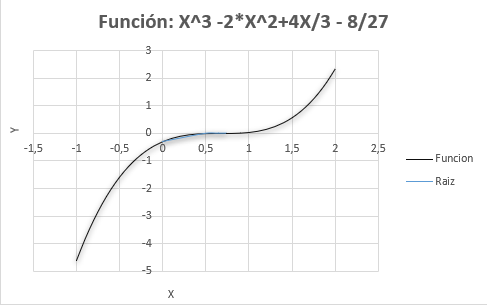
\includegraphics{Captura.PNG}

Grafica 1: Resultados del algoritmo de Brent 
\subsection{Pruebas}
Las pruebas se realizaran con diferentes significancias, ya que variar los intervalos no tiene mucho impacto. Pues si la raíz esta en el intervalo la encontrara y sino simplemente se saldra. Los resultados son los siguientes 

\begin{tabular}{| c | c |}
\hline
Significancia & Raíz \\ \hline
$\epsilon^{-7}$ &   0.6666652  \\
$\epsilon^{-10}$ &  0.6666652109 \\
$\epsilon^{-15}$ & 0.6666652109770974 \\ \hline
\end{tabular}

Tabla 2: Pruebas 

A partir de la talba 2 se concliye quea medida que aumenta la tolerancia el resultado de la raiz es más exacto y tiene una mejor aproximación 

\end{document}
